\chapter{Naive Bayes}
\label{ch:bayes}

Il ragionamento bayesiano è un approccio probabilistico all'inferenza. Si basa sull'assunzione che i dati sono governati da distribuzioni di probabilità e che possono essere prese decisioni ottimali relative a queste probabilità insieme agli esempi a disposizione. Un modello bayesiano non è complicato da costruire, soprattutto su grandi dataset. Nonostante la sua semplicità, tale classificatore spesso si comporta meglio di altri classificatori più sofisticati\cite{Domingos:1997:OSB:274158.274160}.

\section{Teorema di Bayes}
Nel contesto di classificazione, quello che interessa è determinare la migliore ipotesi $h$ appartenente ad uno spazio delle ipotesi $H$ e i dati osservati $D$. Un modo per determinare la \emph{migliore} ipotesi è ricercare la \emph{più probabile}, grazie ai dati a disposizione più una conoscenza iniziale sulle probabilità a priori delle varie ipotesi in $H$\cite{Mitchell:1997:ML:541177}. Il teorema di Bayes fornisce un modo diretto per calcolare queste probabilità, in particolare:

\begin{itemize}
	\item $P(h)$, la \emph{probabilità a priori} che l'ipotesi $h$ sia valida, prima di aver osservato i dati di training. Riflette una qualche conoscenza pregressa che abbiamo circa la possibiltà che $h$ sia corretta.
	\item $P(D)$ denota la priorità a priori che i dati di training $D$ saranno osservati, senza fare alcuna considerazione sulle ipotesi.
	\item $P(D|h)$ denota la probabilità di osservare i dati $D$ in un mondo in cui l'ipotesi $h$ regga.
	\item $P(h|D)$ è la probabilità che $h$ sia valida dopo aver osservato i dati di training $D$. Si tratta della \emph{probabilità a posteriori} di $h$ perché riflette la confidenza che $h$ sia corretta dopo aver visto $D$.
\end{itemize}

Quello che ci interessa è $P(h|D)$, che è possibile calcolare combinando le probabilità succitate:

$$ P(h|D) = \frac{P(D|h) P(h)}{P(D)} $$

Come è facile intuire, $P(h|D)$ aumenta con $P(h)$ e con $P(D|h)$. Analogamente, $P(h|D)$ diminuisce all'aumentare di $P(D)$, perché più è probabile che $D$ venga osservato non considerando $h$, meno evidenza $D$ fornisce in supporto ad $h$.

In molti scenari di apprendimento vengono considerate un insieme $H$ di ipotesi candidate e, tra di esse, ci interessa trovare quella più probabile dopo aver osservato i dati $D$ (o almeno quella massimamente più probabile, se ce n'è più di una). Questa ipotesi è chiamata ipotesi \emph{maximum a posteriori} (MAP). Si può determinare l'ipotesi MAP usando il teorema di Bayes per calcolare la probabilità a posteriori di ogni ipotesi candidata, e poi trovare quella che massimizza tale probabilità:

$$h_{MAP} \equiv \argmax_{h \in H} P(h|D) $$
$$\hphantom{1111111111} = \argmax_{h \in H} \frac{P(D|h) P(h)}{P(D)} $$
$$\hphantom{1111111111} = \argmax_{h \in H} P(D|h) P(h) $$

\noindent
Il termine $P(D)$ può essere tolto perché è una costante indipendente da $h$.

\begin{figure}[htbp!]
	\begin{subfigure}{.5\textwidth}
		\centering
		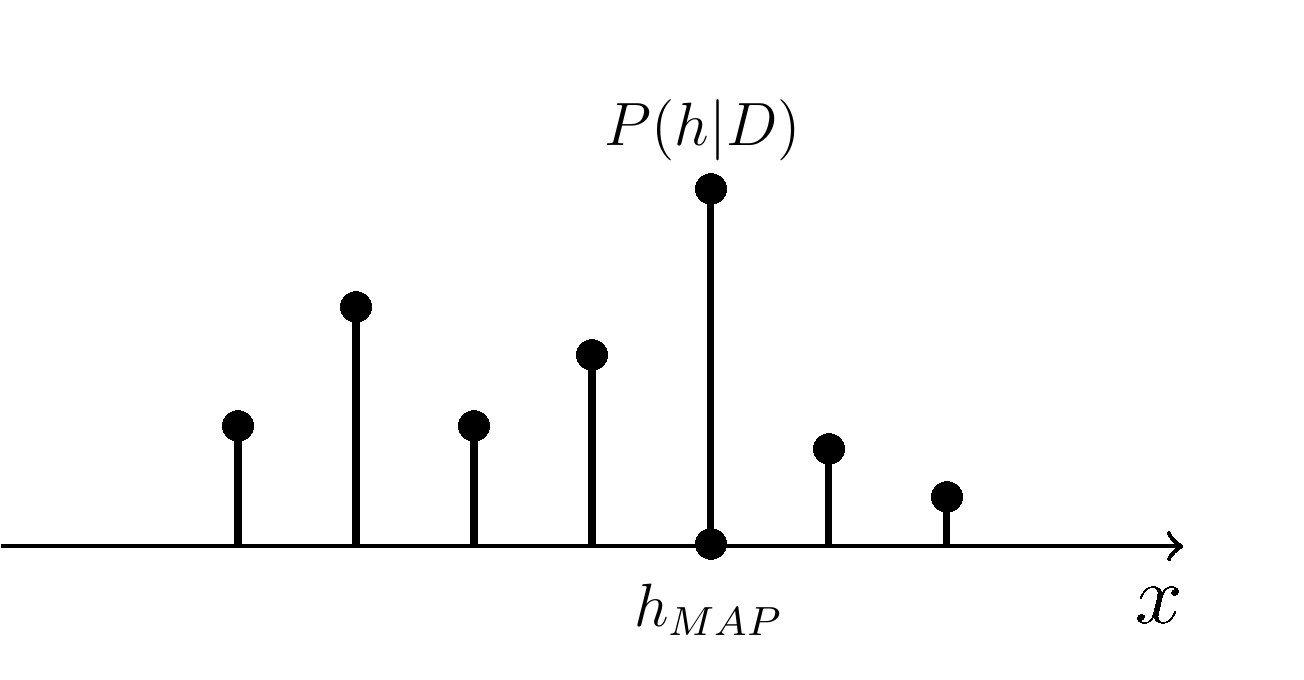
\includegraphics[width=.8\linewidth]{./images/discr}
		\caption{Discreto}
		\label{fig:discr}
	\end{subfigure}
	\begin{subfigure}{.5\textwidth}
		\centering
		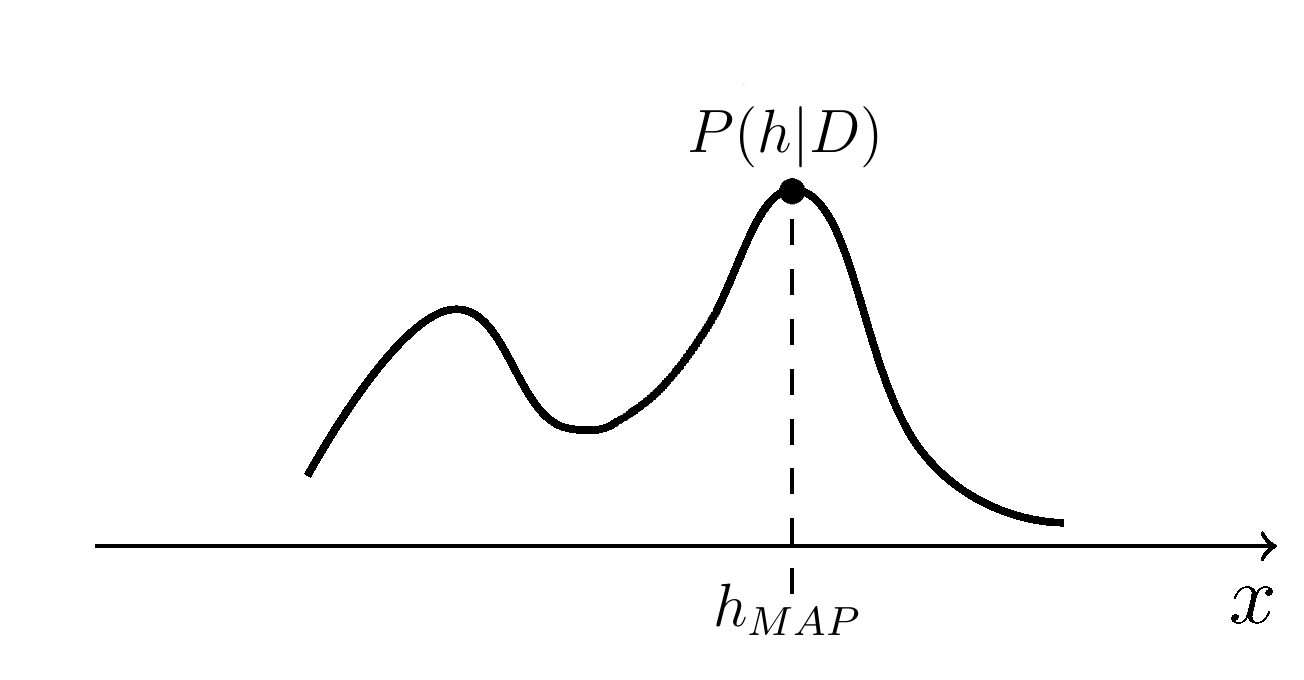
\includegraphics[width=.8\linewidth]{./images/cont}
		\caption{Continuo}
		\label{fig:cont}
	\end{subfigure}
	\caption{Rappresentazione di MAP}
	\label{fig:hmap}
\end{figure}

\section{Naive Bayes Classifier}
Un metodo di apprendimento molto efficace è il classificatore \emph{naive Bayes}. Esso si applica a task di apprendimento in cui ogni istanza è descritta come una congiunzione di valori di attributo $\langle a_1, ..., a_n \rangle$ e dove l'attributo target può assumere qualsiasi valore da un insieme finito $V$.

Ad una nuova istanza viene assegnato il più probabile valore target $v_{MAP}$, considerati i valori di attributo $\langle a_1, ..., a_n \rangle$:

$$ v_{MAP} = \argmax_{v_j \in V} P(v_j | a_1, ..., a_n) $$

Riapplicando le trasformazioni relative alla MAP definite sopra, possiamo riscrivere l'espressione come:

$$v_{MAP} = \argmax_{h \in H} \frac{P(a_1, ..., a_n | v_j) P(v_j)}{P(a_1, ..., a_n)} $$
$$\hphantom{11111} = \argmax_{h \in H} P(a_1, ..., a_n | v_j) P(v_j) $$

Ora bisogna stimare le due probabilità sui dati di training. I vari $P(v_j)$ possono essere facilmente calcolati contando la frequenza con cui ogni valore target $v_j$ occorre nei dati. Non è altrettanto semplice calcolare $P(a_1, ..., a_n | v_j)$ allo stesso modo. Il problema è che ci sono molte probabilità da calcolare e pochi dati a disposizione per ottenere delle stime affidabili: servirebbero dataset molto grandi.

Qui entra in gioco il punto cardine del NBC, ossia presupporre che esista l'\emph{indipendenza condizionale} tra gli attributi. In altre parole, l'assunzione è che, dato il valore target, la probabilità di osservare la congiunzione $a_1, ..., a_n$ è semplicemente il prodotto delle probabilità dei singoli attributi:

$$ P(a_1, ..., a_n | v_j) = \prod_i P(a_i|v_j) $$

\noindent
Facendo le opportune sostituzioni otteniamo:

$$ v_{NB} = v_{MAP} = \argmax_{v_j \in V} P(v_j) \prod_i P(a_i|v_j) $$

dove $v_{NB}$ è il valore target restituito da NBC, che è uguale a $v_{MAP}$ quando si assume l'indipendenza condizionale. Si noti che $P(a_i|v_j)$ è semplicemente il numero dei valori di attributo distinti moltiplicato il numero dei valori target distinti, chiaramente un numero molto più piccolo e gestibile rispetto a $P(a_1, ..., a_n | v_j)$ senza l'ipotesi di indipendenza. 

L'algoritmo di un NBC è pertanto:
\begin{itemize}
	\item Calcola i vari $P(v_j)$ e $P(a_i|v_j)$, basandoti sulle loro frequenze sui dati di training.
	\item Usa queste stime per formare l'ipotesi.
	\item Ogniqualvolta l'assunzione di indipendenza condizionale è soddisfatta, la classificazione $v_{NB}$ è uguale alla classificazione MAP.
\end{itemize}

Un aspetto interessante è che NBC non effettua alcuna ricerca esplicita nello spazio delle ipotesi. Viene costruita l'ipotesi semplicemente contando le frequenze delle varie combinazioni dei dati all'interno del training set.

\subsection*{Attributi continui}
Contare le frequenze delle diverse combinazioni di valori è possibile per gli attributi discreti, quindi bisogna trovare un modo per calcolare le probabilità degli eventuali attributi continui. Ci sono due strade: la prima è appunto discretizzare i valori numerici in vari \emph{bin}, l'altra è assumere l'esistenza di una distribuzione normale (Gaussiana) per i valori $\langle a_1, ..., a_n \rangle$ dell'attributo $A_k$. Questa funzione ha bisogno di due parametri, media e deviazione standard degli attributi:

$$ \mu_{kj} = E[A_k | v_j] = \frac{1}{n} \sum_{i = 1}^{n} a_i$$
$$ \sigma_{kj} = \sqrt{ E[(A_k - \mu_{kj})^2 | v_j] } = \sqrt{ \frac{1}{n-1} \sum_{i = 1}^{n} (a_i - \mu_{kj})^2 } $$

Infine, serve la funzione di densità di probabilità della Gaussiana, che applicata al nostro contesto diventa:

$$ P(a_i | v_j) = \frac{1}{\sigma\sqrt{2\pi}} e^{-\frac{(a_i-\mu)^2}{2\sigma^2}} $$
